% Generated by make_figures.py; do not edit by hand.

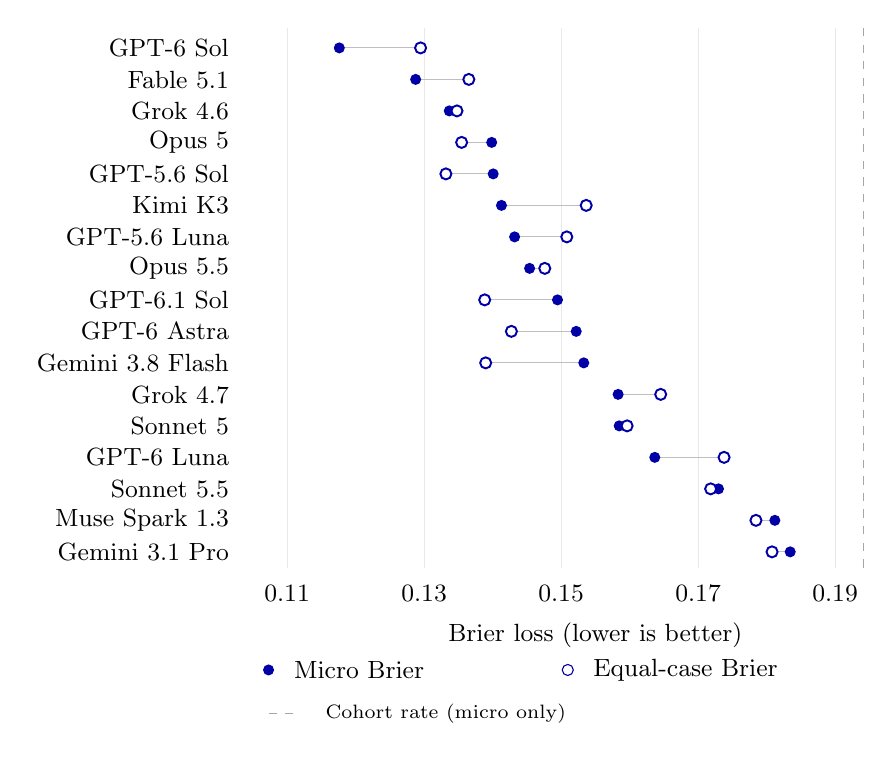
\begin{tikzpicture}[every node/.style={font=\small}]
\draw[gray!18] (0.43500,-.2)--(0.43500,6.65000);
\node[anchor=north] at (0.43500,-.3) {0.11};
\draw[gray!18] (2.17500,-.2)--(2.17500,6.65000);
\node[anchor=north] at (2.17500,-.3) {0.13};
\draw[gray!18] (3.91500,-.2)--(3.91500,6.65000);
\node[anchor=north] at (3.91500,-.3) {0.15};
\draw[gray!18] (5.65500,-.2)--(5.65500,6.65000);
\node[anchor=north] at (5.65500,-.3) {0.17};
\draw[gray!18] (7.39500,-.2)--(7.39500,6.65000);
\node[anchor=north] at (7.39500,-.3) {0.19};
\draw[dashed,gray!70] (7.75160,-.2)--(7.75160,6.65000);
\node[anchor=east] at (-.18,0.000) {Gemini 3.1 Pro};
\draw[gray!50] (6.82512,0.000)--(6.59447,0.000);
\fill[blue!65!black] (6.82512,0.000) circle (2pt);
\draw[blue!65!black,fill=white,line width=.7pt] (6.59447,0.000) circle (2pt);
\node[anchor=east] at (-.18,0.400) {Muse Spark 1.3};
\draw[gray!50] (6.62998,0.400)--(6.38993,0.400);
\fill[blue!65!black] (6.62998,0.400) circle (2pt);
\draw[blue!65!black,fill=white,line width=.7pt] (6.38993,0.400) circle (2pt);
\node[anchor=east] at (-.18,0.800) {Sonnet 5.5};
\draw[gray!50] (5.91407,0.800)--(5.81460,0.800);
\fill[blue!65!black] (5.91407,0.800) circle (2pt);
\draw[blue!65!black,fill=white,line width=.7pt] (5.81460,0.800) circle (2pt);
\node[anchor=east] at (-.18,1.200) {GPT-6 Luna};
\draw[gray!50] (5.10507,1.200)--(5.98509,1.200);
\fill[blue!65!black] (5.10507,1.200) circle (2pt);
\draw[blue!65!black,fill=white,line width=.7pt] (5.98509,1.200) circle (2pt);
\node[anchor=east] at (-.18,1.600) {Sonnet 5};
\draw[gray!50] (4.65311,1.600)--(4.75361,1.600);
\fill[blue!65!black] (4.65311,1.600) circle (2pt);
\draw[blue!65!black,fill=white,line width=.7pt] (4.75361,1.600) circle (2pt);
\node[anchor=east] at (-.18,2.000) {Grok 4.7};
\draw[gray!50] (4.63933,2.000)--(5.18010,2.000);
\fill[blue!65!black] (4.63933,2.000) circle (2pt);
\draw[blue!65!black,fill=white,line width=.7pt] (5.18010,2.000) circle (2pt);
\node[anchor=east] at (-.18,2.400) {Gemini 3.8 Flash};
\draw[gray!50] (4.20331,2.400)--(2.95760,2.400);
\fill[blue!65!black] (4.20331,2.400) circle (2pt);
\draw[blue!65!black,fill=white,line width=.7pt] (2.95760,2.400) circle (2pt);
\node[anchor=east] at (-.18,2.800) {GPT-6 Astra};
\draw[gray!50] (4.10730,2.800)--(3.28403,2.800);
\fill[blue!65!black] (4.10730,2.800) circle (2pt);
\draw[blue!65!black,fill=white,line width=.7pt] (3.28403,2.800) circle (2pt);
\node[anchor=east] at (-.18,3.200) {GPT-6.1 Sol};
\draw[gray!50] (3.86964,3.200)--(2.94516,3.200);
\fill[blue!65!black] (3.86964,3.200) circle (2pt);
\draw[blue!65!black,fill=white,line width=.7pt] (2.94516,3.200) circle (2pt);
\node[anchor=east] at (-.18,3.600) {Opus 5.5};
\draw[gray!50] (3.51502,3.600)--(3.70814,3.600);
\fill[blue!65!black] (3.51502,3.600) circle (2pt);
\draw[blue!65!black,fill=white,line width=.7pt] (3.70814,3.600) circle (2pt);
\node[anchor=east] at (-.18,4.000) {GPT-5.6 Luna};
\draw[gray!50] (3.32487,4.000)--(3.98765,4.000);
\fill[blue!65!black] (3.32487,4.000) circle (2pt);
\draw[blue!65!black,fill=white,line width=.7pt] (3.98765,4.000) circle (2pt);
\node[anchor=east] at (-.18,4.400) {Kimi K3};
\draw[gray!50] (3.15799,4.400)--(4.23419,4.400);
\fill[blue!65!black] (3.15799,4.400) circle (2pt);
\draw[blue!65!black,fill=white,line width=.7pt] (4.23419,4.400) circle (2pt);
\node[anchor=east] at (-.18,4.800) {GPT-5.6 Sol};
\draw[gray!50] (3.05295,4.800)--(2.45220,4.800);
\fill[blue!65!black] (3.05295,4.800) circle (2pt);
\draw[blue!65!black,fill=white,line width=.7pt] (2.45220,4.800) circle (2pt);
\node[anchor=east] at (-.18,5.200) {Opus 5};
\draw[gray!50] (3.03378,5.200)--(2.65210,5.200);
\fill[blue!65!black] (3.03378,5.200) circle (2pt);
\draw[blue!65!black,fill=white,line width=.7pt] (2.65210,5.200) circle (2pt);
\node[anchor=east] at (-.18,5.600) {Grok 4.6};
\draw[gray!50] (2.49521,5.600)--(2.59299,5.600);
\fill[blue!65!black] (2.49521,5.600) circle (2pt);
\draw[blue!65!black,fill=white,line width=.7pt] (2.59299,5.600) circle (2pt);
\node[anchor=east] at (-.18,6.000) {Fable 5.1};
\draw[gray!50] (2.06804,6.000)--(2.74354,6.000);
\fill[blue!65!black] (2.06804,6.000) circle (2pt);
\draw[blue!65!black,fill=white,line width=.7pt] (2.74354,6.000) circle (2pt);
\node[anchor=east] at (-.18,6.400) {GPT-6 Sol};
\draw[gray!50] (1.09863,6.400)--(2.13074,6.400);
\fill[blue!65!black] (1.09863,6.400) circle (2pt);
\draw[blue!65!black,fill=white,line width=.7pt] (2.13074,6.400) circle (2pt);
\node[anchor=north] at (4.35,-.78) {Brier loss (lower is better)};
\fill[blue!65!black] (.2,-1.5) circle(2pt);\node[anchor=west] at (.4,-1.5) {Micro Brier};
\draw[blue!65!black,fill=white] (4.0,-1.5) circle(2pt);\node[anchor=west] at (4.2,-1.5) {Equal-case Brier};
\draw[dashed,gray!70] (.2,-2.05)--(.6,-2.05);\node[anchor=west,font=\scriptsize] at (.8,-2.05) {Cohort rate (micro only)};\end{tikzpicture}

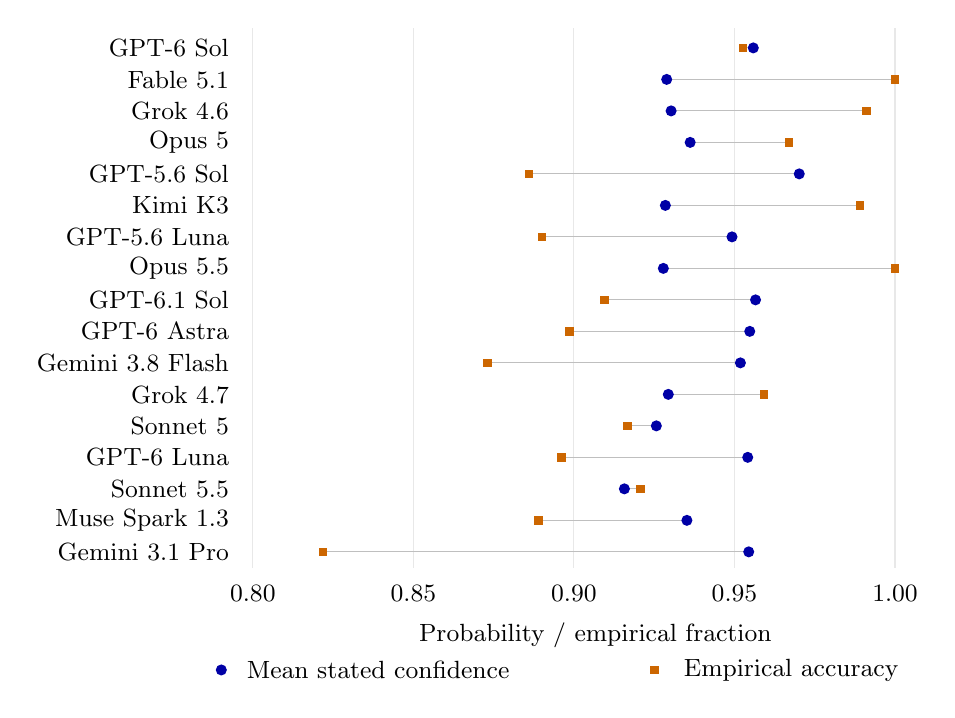
\begin{tikzpicture}[every node/.style={font=\small}]
\draw[gray!18] (0.00000,-.2)--(0.00000,6.65000);
\node[anchor=north] at (0.00000,-.3) {0.80};
\draw[gray!18] (2.03906,-.2)--(2.03906,6.65000);
\node[anchor=north] at (2.03906,-.3) {0.85};
\draw[gray!18] (4.07812,-.2)--(4.07812,6.65000);
\node[anchor=north] at (4.07812,-.3) {0.90};
\draw[gray!18] (6.11719,-.2)--(6.11719,6.65000);
\node[anchor=north] at (6.11719,-.3) {0.95};
\draw[gray!18] (8.15625,-.2)--(8.15625,6.65000);
\node[anchor=north] at (8.15625,-.3) {1.00};
\node[anchor=east] at (-.18,0.000) {Gemini 3.1 Pro};
\draw[gray!50] (6.29815,0.000)--(0.89209,0.000);
\fill[blue!65!black] (6.29815,0.000) circle (2pt);
\fill[orange!80!black] (0.83709,-0.055) rectangle (0.94709,0.055);
\node[anchor=east] at (-.18,0.400) {Muse Spark 1.3};
\draw[gray!50] (5.51302,0.400)--(3.62500,0.400);
\fill[blue!65!black] (5.51302,0.400) circle (2pt);
\fill[orange!80!black] (3.57000,0.345) rectangle (3.68000,0.455);
\node[anchor=east] at (-.18,0.800) {Sonnet 5.5};
\draw[gray!50] (4.71897,0.800)--(4.91964,0.800);
\fill[blue!65!black] (4.71897,0.800) circle (2pt);
\fill[orange!80!black] (4.86464,0.745) rectangle (4.97464,0.855);
\node[anchor=east] at (-.18,1.200) {GPT-6 Luna};
\draw[gray!50] (6.28544,1.200)--(3.92213,1.200);
\fill[blue!65!black] (6.28544,1.200) circle (2pt);
\fill[orange!80!black] (3.86713,1.145) rectangle (3.97713,1.255);
\node[anchor=east] at (-.18,1.600) {Sonnet 5};
\draw[gray!50] (5.12484,1.600)--(4.75781,1.600);
\fill[blue!65!black] (5.12484,1.600) circle (2pt);
\fill[orange!80!black] (4.70281,1.545) rectangle (4.81281,1.655);
\node[anchor=east] at (-.18,2.000) {Grok 4.7};
\draw[gray!50] (5.27659,2.000)--(6.49171,2.000);
\fill[blue!65!black] (5.27659,2.000) circle (2pt);
\fill[orange!80!black] (6.43671,1.945) rectangle (6.54671,2.055);
\node[anchor=east] at (-.18,2.400) {Gemini 3.8 Flash};
\draw[gray!50] (6.19254,2.400)--(2.98471,2.400);
\fill[blue!65!black] (6.19254,2.400) circle (2pt);
\fill[orange!80!black] (2.92971,2.345) rectangle (3.03971,2.455);
\node[anchor=east] at (-.18,2.800) {GPT-6 Astra};
\draw[gray!50] (6.31124,2.800)--(4.01902,2.800);
\fill[blue!65!black] (6.31124,2.800) circle (2pt);
\fill[orange!80!black] (3.96402,2.745) rectangle (4.07402,2.855);
\node[anchor=east] at (-.18,3.200) {GPT-6.1 Sol};
\draw[gray!50] (6.38462,3.200)--(4.46749,3.200);
\fill[blue!65!black] (6.38462,3.200) circle (2pt);
\fill[orange!80!black] (4.41249,3.145) rectangle (4.52249,3.255);
\node[anchor=east] at (-.18,3.600) {Opus 5.5};
\draw[gray!50] (5.21373,3.600)--(8.15625,3.600);
\fill[blue!65!black] (5.21373,3.600) circle (2pt);
\fill[orange!80!black] (8.10125,3.545) rectangle (8.21125,3.655);
\node[anchor=east] at (-.18,4.000) {GPT-5.6 Luna};
\draw[gray!50] (6.08582,4.000)--(3.67479,4.000);
\fill[blue!65!black] (6.08582,4.000) circle (2pt);
\fill[orange!80!black] (3.61979,3.945) rectangle (3.72979,4.055);
\node[anchor=east] at (-.18,4.400) {Kimi K3};
\draw[gray!50] (5.23950,4.400)--(7.71298,4.400);
\fill[blue!65!black] (5.23950,4.400) circle (2pt);
\fill[orange!80!black] (7.65798,4.345) rectangle (7.76798,4.455);
\node[anchor=east] at (-.18,4.800) {GPT-5.6 Sol};
\draw[gray!50] (6.93979,4.800)--(3.50576,4.800);
\fill[blue!65!black] (6.93979,4.800) circle (2pt);
\fill[orange!80!black] (3.45076,4.745) rectangle (3.56076,4.855);
\node[anchor=east] at (-.18,5.200) {Opus 5};
\draw[gray!50] (5.55434,5.200)--(6.80811,5.200);
\fill[blue!65!black] (5.55434,5.200) circle (2pt);
\fill[orange!80!black] (6.75311,5.145) rectangle (6.86311,5.255);
\node[anchor=east] at (-.18,5.600) {Grok 4.6};
\draw[gray!50] (5.31249,5.600)--(7.79213,5.600);
\fill[blue!65!black] (5.31249,5.600) circle (2pt);
\fill[orange!80!black] (7.73713,5.545) rectangle (7.84713,5.655);
\node[anchor=east] at (-.18,6.000) {Fable 5.1};
\draw[gray!50] (5.25625,6.000)--(8.15625,6.000);
\fill[blue!65!black] (5.25625,6.000) circle (2pt);
\fill[orange!80!black] (8.10125,5.945) rectangle (8.21125,6.055);
\node[anchor=east] at (-.18,6.400) {GPT-6 Sol};
\draw[gray!50] (6.35608,6.400)--(6.22578,6.400);
\fill[blue!65!black] (6.35608,6.400) circle (2pt);
\fill[orange!80!black] (6.17078,6.345) rectangle (6.28078,6.455);
\node[anchor=north] at (4.35,-.78) {Probability / empirical fraction};
\fill[blue!65!black] (-.4,-1.5) circle(2pt);\node[anchor=west] at (-.2,-1.5) {Mean stated confidence};
\fill[orange!80!black] (5.05,-1.555) rectangle(5.16,-1.445);\node[anchor=west] at (5.35,-1.5) {Empirical accuracy};\end{tikzpicture}

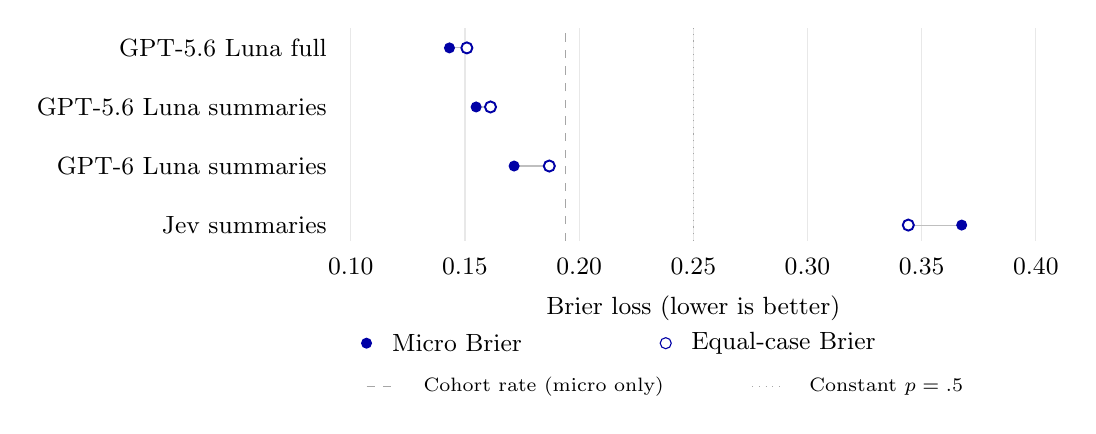
\begin{tikzpicture}[every node/.style={font=\small}]
\draw[gray!18] (0.00000,-.2)--(0.00000,2.500);
\node[anchor=north] at (0.00000,-.3) {0.10};
\draw[gray!18] (1.45000,-.2)--(1.45000,2.500);
\node[anchor=north] at (1.45000,-.3) {0.15};
\draw[gray!18] (2.90000,-.2)--(2.90000,2.500);
\node[anchor=north] at (2.90000,-.3) {0.20};
\draw[gray!18] (4.35000,-.2)--(4.35000,2.500);
\node[anchor=north] at (4.35000,-.3) {0.25};
\draw[gray!18] (5.80000,-.2)--(5.80000,2.500);
\node[anchor=north] at (5.80000,-.3) {0.30};
\draw[gray!18] (7.25000,-.2)--(7.25000,2.500);
\node[anchor=north] at (7.25000,-.3) {0.35};
\draw[gray!18] (8.70000,-.2)--(8.70000,2.500);
\node[anchor=north] at (8.70000,-.3) {0.40};
\draw[dashed,gray!70] (2.72887,-.2)--(2.72887,2.500);
\draw[dotted,gray!70] (4.35000,-.2)--(4.35000,2.500);
\node[anchor=east] at (-.18,0.000) {Jev summaries};
\draw[gray!50] (7.75870,0.000)--(7.08070,0.000);
\fill[blue!65!black] (7.75870,0.000) circle (2pt);
\draw[blue!65!black,fill=white,line width=.7pt] (7.08070,0.000) circle (2pt);
\node[anchor=east] at (-.18,0.750) {GPT-6 Luna summaries};
\draw[gray!50] (2.07411,0.750)--(2.52134,0.750);
\fill[blue!65!black] (2.07411,0.750) circle (2pt);
\draw[blue!65!black,fill=white,line width=.7pt] (2.52134,0.750) circle (2pt);
\node[anchor=east] at (-.18,1.500) {GPT-5.6 Luna summaries};
\draw[gray!50] (1.59194,1.500)--(1.77464,1.500);
\fill[blue!65!black] (1.59194,1.500) circle (2pt);
\draw[blue!65!black,fill=white,line width=.7pt] (1.77464,1.500) circle (2pt);
\node[anchor=east] at (-.18,2.250) {GPT-5.6 Luna full};
\draw[gray!50] (1.25329,2.250)--(1.47422,2.250);
\fill[blue!65!black] (1.25329,2.250) circle (2pt);
\draw[blue!65!black,fill=white,line width=.7pt] (1.47422,2.250) circle (2pt);
\node[anchor=north] at (4.35,-.78) {Brier loss (lower is better)};
\fill[blue!65!black] (.2,-1.5) circle(2pt);\node[anchor=west] at (.4,-1.5) {Micro Brier};
\draw[blue!65!black,fill=white] (4.0,-1.5) circle(2pt);\node[anchor=west] at (4.2,-1.5) {Equal-case Brier};
\draw[dashed,gray!70] (.2,-2.05)--(.6,-2.05);\node[anchor=west,font=\scriptsize] at (.8,-2.05) {Cohort rate (micro only)};\draw[dotted,gray!70] (5.1,-2.05)--(5.5,-2.05);\node[anchor=west,font=\scriptsize] at (5.7,-2.05) {Constant $p=.5$};\end{tikzpicture}
